\documentclass[a4paper,11pt]{report}
\usepackage[utf8]{inputenc}
\usepackage[T1]{fontenc}
\usepackage{lmodern}
\usepackage[ngerman]{babel}
\usepackage[margin=20mm, left=20mm, right=10mm, headheight=15pt, includeheadfoot]{geometry}
\usepackage{fancyhdr}
\usepackage{opensans}
\usepackage{titlesec}
\usepackage{tocloft}
\usepackage{titling}
\usepackage{hyperref}
\usepackage{graphicx}
\usepackage{enumerate}
\usepackage{float}
\usepackage{caption}
\usepackage{listings}
\usepackage{minted}
\usepackage{subcaption}
\usepackage{enumitem}
\usemintedstyle{vs}

% Author and subject
\author{Felix Hillebrand}
\newcommand{\subject}{SSD4UE}

\graphicspath{ {./images/} }

% Set default font to OpenSans
\renewcommand*\familydefault{\sfdefault}

% Page style for cover page
\fancypagestyle{cover}{
    \fancyhf{}
    \renewcommand{\headrulewidth}{0pt}
    \renewcommand{\footrulewidth}{0pt}
}

% Page style for main content
\fancypagestyle{main}{
    \fancyhf{}
    \fancyhead[L]{\theauthor}
    \fancyhead[R]{\subject}
    \fancyfoot[C]{\thepage}
    \renewcommand{\headrulewidth}{0.4pt}
    \renewcommand{\footrulewidth}{0pt}
}

\titleformat{\chapter}[block]
  {\normalfont\Large\bfseries} % change \Large to \large or any other size that fits
  {\thechapter}
  {1em}
  {}

  \titlespacing*{\chapter}{0pt}{*4}{*2.5}

% Cover page
\newcommand{\coverpage}{
    \thispagestyle{cover}
    \begin{center}
        % {
\includegraphics[height=3cm]{fh-logo.png}}\\[1cm]
        {\LARGE \thetitle}\\[0.5cm]
        {\large \theauthor}\\
        \href{mailto:97hilfel@gmail.com}{97hilfel@gmail.com}\\
    \end{center}
    \tableofcontents
    \clearpage
}

\newcommand{\screenshot}[1]{
    \begin{figure}[H]
        \centering
        \includegraphics[scale=0.375]{#1}
    \end{figure}
}

% Main document
\begin{document}

% Color definitions
\definecolor{LightGray}{gray}{0.9}
\definecolor{DarkGray}{gray}{0.3}

\title{AMS4~-~U02}
\coverpage

\pagenumbering{roman}
\clearpage
\pagenumbering{arabic}
\pagestyle{main}

\chapter{Bipartite Graphen}
    \begin{description}
        \item[Aufgabe:] Bestimmen Sie für die Graphen A, B und C ob es sich um bipartite Graphen handelt, und geben sie falls möglich zei Knotenmegen an. \hfill
        \begin{figure}[htbp]
            \centering
            \begin{subfigure}[b]{0.3\textwidth}
                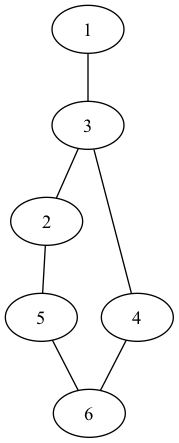
\includegraphics[height=0.2\textheight]{notebooks/assets/aufgabe_01/A}
                \caption{A}
                \label{fig:a01_a}
            \end{subfigure}
            \hfill
            \begin{subfigure}[b]{0.3\textwidth}
                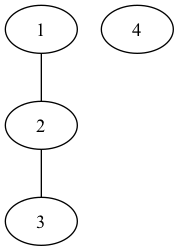
\includegraphics[height=0.2\textheight]{notebooks/assets/aufgabe_01/B}
                \caption{B}
                \label{fig:a01_b}
            \end{subfigure}
            \hfill
            \begin{subfigure}[b]{0.3\textwidth}
                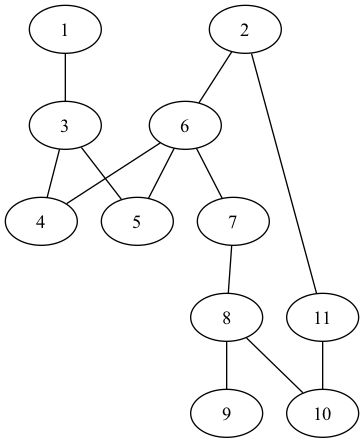
\includegraphics[height=0.2\textheight]{notebooks/assets/aufgabe_01/C}
                \caption{C}
                \label{fig:a01_c}
            \end{subfigure}
            \hfill
        \end{figure}
        \item[Lösung:] \hfill \newline % Use hfill to move the figure to the next line
        \begin{figure}[htbp]
            \centering
            \begin{subfigure}[b]{0.3\textwidth}
                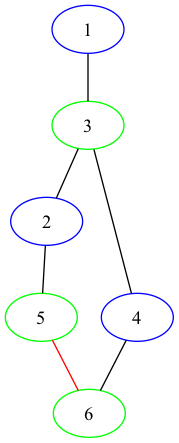
\includegraphics[height=0.2\textheight]{notebooks/assets/aufgabe_01/A_colored}
                \caption{A - nicht Bipartit - Kante $\{5, 6\}$}
                \label{fig:a01_a_colored}
            \end{subfigure}
            \hfill
            \begin{subfigure}[b]{0.3\textwidth}
                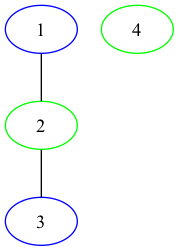
\includegraphics[height=0.2\textheight]{notebooks/assets/aufgabe_01/B_colored}
                \caption{B - Bipartit}
                \label{fig:a01_b_colored}
            \end{subfigure}
            \hfill
            \begin{subfigure}[b]{0.3\textwidth}
                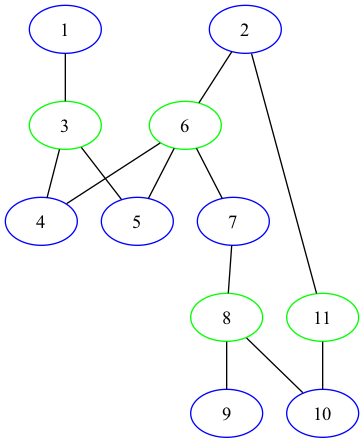
\includegraphics[height=0.2\textheight]{notebooks/assets/aufgabe_01/C_colored}
                \caption{C - Bipartit}
                \label{fig:a01_c_colored}
            \end{subfigure}
            \hfill
        \end{figure}

    \end{description}
\newpage

\chapter{Topologisches Sortieren}
Ein prominentes Beispiel für das Erkennen von Zyklen ist das Serialisieren von Transaktionen in Datenbanksystemen.
In der untenstehenden Tabelle ist der vom DBMS registrierte Ablaufplan angegeben.
Transformieren Sie den Plan in einen gerichteten Graphen, der die Abhängigkeiten zwischen den Transaktionen abbildet und ermitteln Sie ob ein äquivalenter serieller Ablaufplan
(Serie von Transaktionen ohne Verzahnung)
existiert und geben Sie gegeben falls einen möglichen an.

\textbf{Hinweis}: Gegeben 2 Transaktionen \texttt{a} und \texttt{b} $a != b$ und eine Tabelle X so gilt:

\begin{itemize}
    \item wenn \texttt{R, a, X} vor \texttt{W, b, X} dann \texttt{a} vor \texttt{b} im seriellen Plan)
    \item wenn \texttt{W, a, X} vor \texttt{R, b, X} dann \texttt{a} vor \texttt{b} im seriellen Plan)
    \item wenn \texttt{W, a, X} vor \texttt{W, b, X} dann \texttt{a} vor \texttt{b} im seriellen Plan)
\end{itemize}

\begin{table}[]
    \begin{tabular}{|l|l|l|l|}
        \hline
        Id & AT & Tx & Table \\ \hline
        1  & R  & 1  & A     \\ \hline
        2  & W  & 1  & A     \\ \hline
        3  & R  & 7  & B     \\ \hline
        4  & R  & 2  & A     \\ \hline
        5  & W  & 2  & A     \\ \hline
        6  & R  & 1  & B     \\ \hline
        7  & W  & 1  & B     \\ \hline
        8  & R  & 2  & B     \\ \hline
        9  & W  & 2  & B     \\ \hline
        10 & R  & 3  & A     \\ \hline
        11 & W  & 4  & A     \\ \hline
        12 & R  & 5  & B     \\ \hline
        13 & R  & 1  & C     \\ \hline
        14 & R  & 6  & C     \\ \hline
        15 & W  & 8  & A     \\ \hline
        16 & W  & 8  & B     \\ \hline
    \end{tabular}
\end{table}

\begin{figure}[]
\end{figure}

\chapter{Legal}
Die Ausarbeitung der Aufgabe wurde durch \texttt{OpenAI - GPT-4.5 Turbo}, \texttt{OpenAI - GPT-4.5 Vision}, \texttt{Anthropic -- Claude 3 Opus},  \texttt{Kagi - FastGPT} mit mehreren unterschiedlichen Prompts und Custom Instructions unterstützt.

\end{document}